\section{Additional results}
\label{app:extra}

\begin{figure*}[t]
\centering
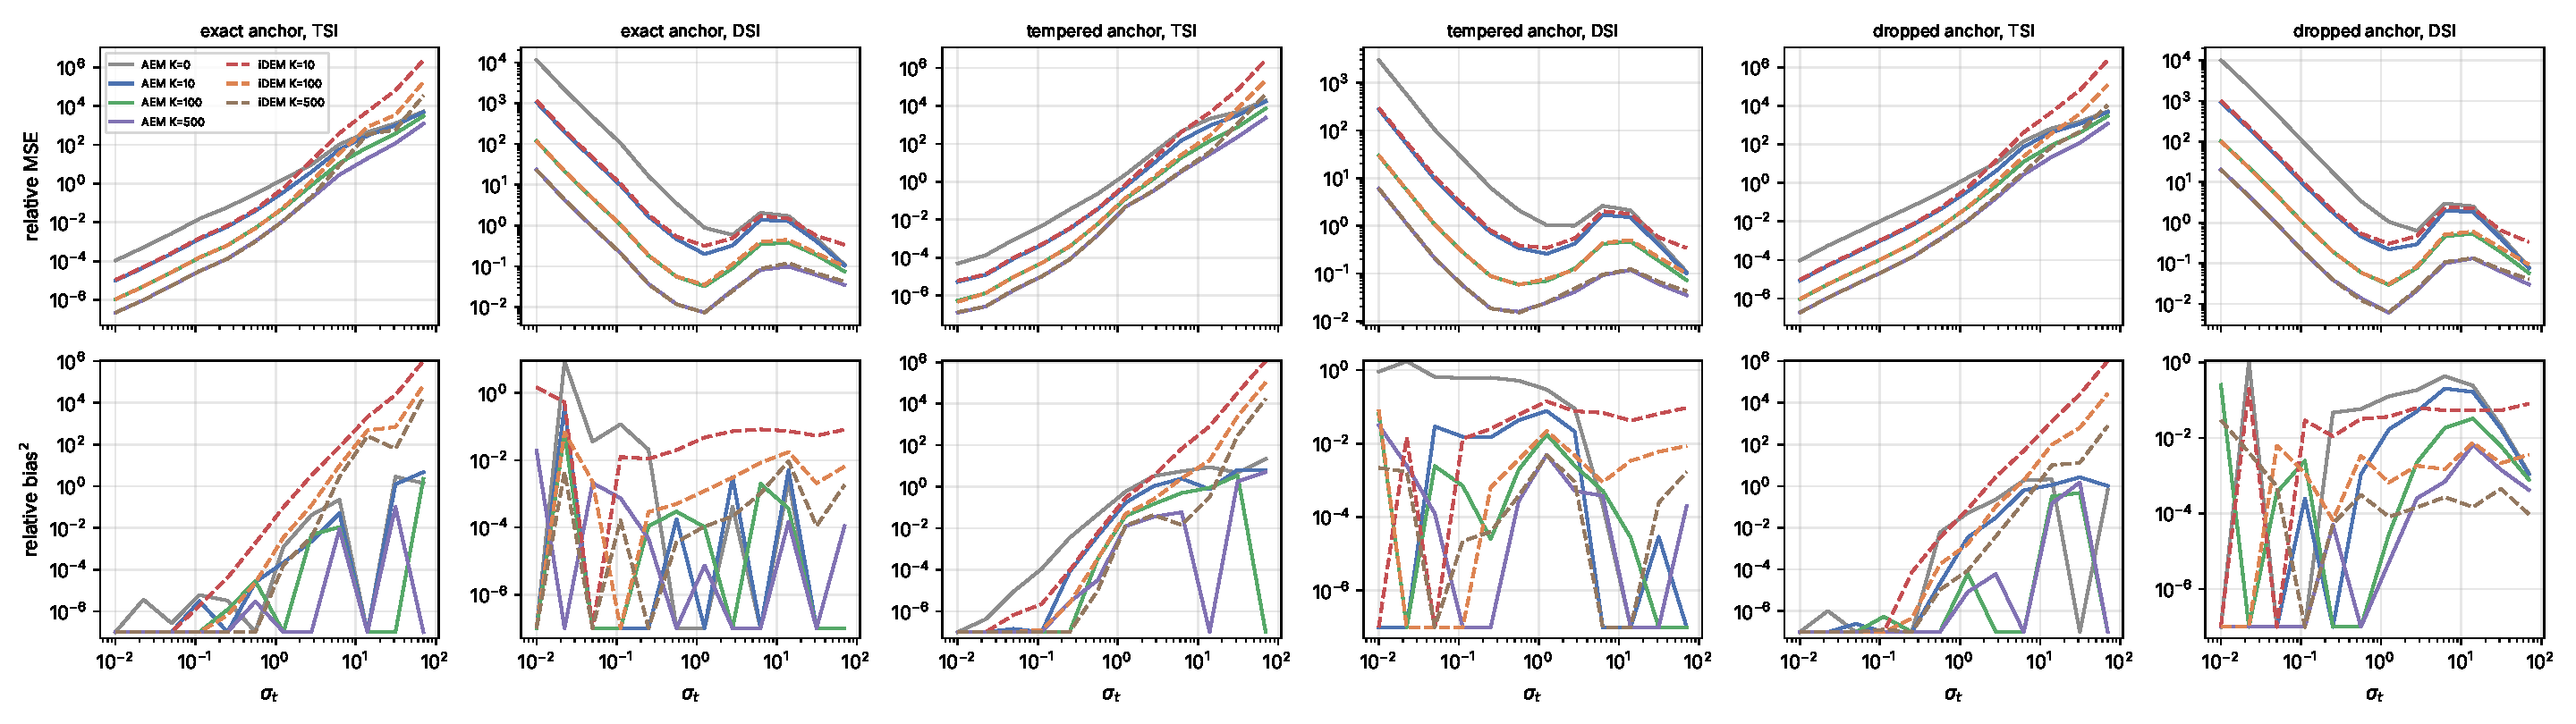
\includegraphics[width=\textwidth]{fig_estimator_gmm40.pdf}
\caption{\textbf{Estimator study on GMM-40.} Relative MSE (top) and debiased relative squared bias (bottom) of the noised-score target against $\sigma_t$, for iDEM (dashed) and AEM (solid) with TSI or DSI test functions. Columns use exact anchors (left), anchors from a tempered target (centre) and anchors from a target missing half of its modes (right). With exact anchors AEM is unbiased for every $K$, including $K=0$. iDEM's bias grows by orders of magnitude with $\sigma_t$.}
\label{fig:estimator}
\end{figure*}

\begin{figure*}[t]
\centering
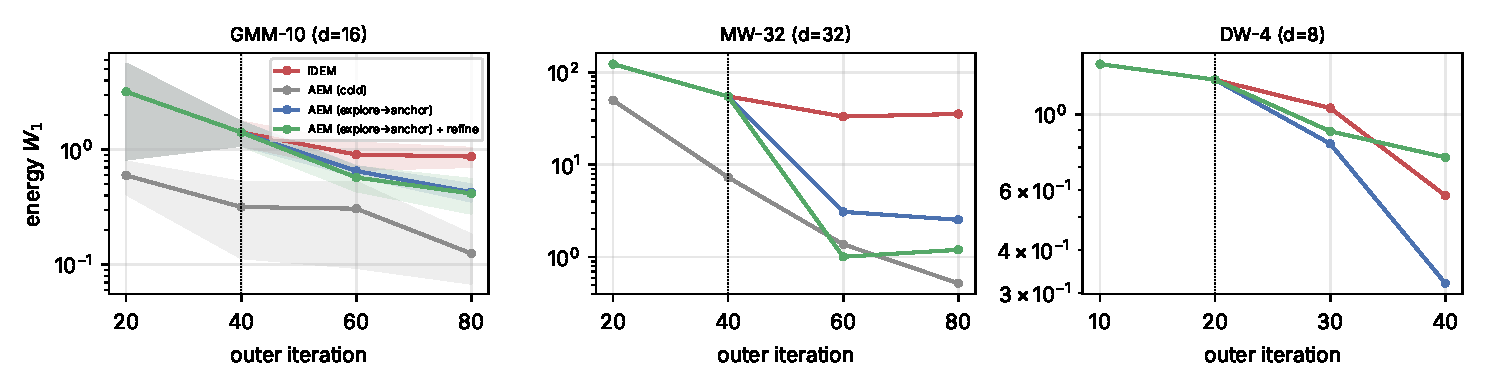
\includegraphics[width=\textwidth,height=0.17\textheight,keepaspectratio]{fig_curves_gpu.pdf}
\caption{\textbf{Energy $\mathcal{W}_1$ during training} (mean and min--max over 3 seeds; log scale). The dotted line marks the switch from exploration to anchoring in the explore$\to$anchor runs. Before it, those runs coincide with iDEM. On LJ-13 the untrimmed metric is dominated by rare very-high-energy samples.}
\label{fig:curves}
\end{figure*}

\paragraph{Replay proposals at the estimator level.}
\Cref{tab:replay} compares four estimators on GMM-10 ($d=16$, $K=100$, precision-weighted test function, 128 points, 8 repeats). The four are iDEM, AEM with Gaussian proposals, replay-SNIS without an anchor, and AEM with replay proposals. Three buffers are used: exact; \emph{skewed}, where half of the modes are over-represented $4{:}1$; and \emph{dropped}, where half of the modes are missing. The anchors and the replay reference set come from the buffer.
At low noise all estimators are essentially exact, because the precision-weighted test function has zero variance within a unit Gaussian component.
At high noise, replay proposals reduce the MSE $2$--$4\times$ compared with Gaussian proposals.
With a skewed buffer, combining the anchor with replay proposals gives the smallest bias at $\sigma_t\approx9.4$ ($1.9\cdot10^{-3}$ vs.\ $9.7\cdot10^{-3}$ for iDEM): the importance weights correct the over-represented modes.
With a dropped buffer, every buffer-informed estimator inherits the missing modes at high noise (bias $\approx4.7\cdot10^{-2}$ vs.\ $4.3\cdot10^{-3}$ for iDEM). This is the exploration limitation discussed in \cref{sec:exp-ablation}.

\begin{table}[h]
\centering
\caption{Relative MSE (relative squared bias in parentheses) of the score target on GMM-10 ($d=16$) at high noise.}
\label{tab:replay}
\small
\begin{tabular}{llcccc}
\toprule
buffer & $\sigma_t$ & iDEM & AEM & replay & AEM + replay\\
\midrule
exact & 4.4 & 5.8e-2 (7.8e-3) & 2.3e-2 (0) & 6.5e-3 (7.8e-4) & 1.4e-2 (0)\\
exact & 9.4 & 1.5e-1 (1.3e-2) & 9.9e-2 (5.5e-4) & 3.6e-2 (0) & 4.7e-2 (0)\\
skewed & 4.4 & 3.4e-2 (4.1e-3) & 2.1e-2 (2.5e-3) & 7.4e-3 (8.4e-4) & 1.0e-2 (5.8e-4)\\
skewed & 9.4 & 1.7e-1 (9.7e-3) & 1.1e-1 (8.9e-3) & 4.5e-2 (7.7e-3) & 5.6e-2 (1.9e-3)\\
dropped & 4.4 & 3.6e-2 (4.3e-3) & 1.3e-2 (4.2e-4) & 3.3e-3 (5.2e-4) & 6.2e-3 (1.3e-4)\\
dropped & 9.4 & 1.4e-1 (4.3e-3) & 1.1e-1 (4.7e-2) & 6.5e-2 (4.6e-2) & 6.9e-2 (4.7e-2)\\
\bottomrule
\end{tabular}
\end{table}

\paragraph{Cold-start ablations (single seed, GMM-10, $d=16$).}
After 10 outer iterations, replay proposals used from the start collapse onto the buffer's modes: iDEM with replay covers $2/10$ modes (mode TV $0.90$), and AEM with replay also covers $2/10$ (mode TV $0.90$). Plain iDEM covers $8/10$ (mode TV $0.59$) and cold AEM $5/10$ (mode TV $0.70$).
This motivates switching replay on only in the anchored phase of explore$\to$anchor training, as we do for AEM-R.

\paragraph{Dimension sweep with non-unit components.}
\Cref{tab:dimsweep} reports the estimator study for 10-component mixtures with component standard deviation $1.5$ and means uniform in $[-10,10]^d$. It uses the TSI/DSI combination from training, $K=100$, 128 points and 16 repeats with exact anchors.

\begin{table}[h]
\centering
\caption{Relative MSE (relative squared bias) of the training test function, and AEM's mean anchor weight, against dimension.}
\label{tab:dimsweep}
\small
\begin{tabular}{rrccc}
\toprule
$d$ & $\sigma_t$ & iDEM & AEM & anchor wt.\\
\midrule
2 & 3 & 3.3e-2 (1.2e-3) & 2.7e-2 (0) & 0.05\\
2 & 10 & 2.9e-2 (4.6e-4) & 2.4e-2 (0) & 0.13\\
8 & 3 & 1.2e-1 (2.0e-2) & 8.9e-2 (0) & 0.81\\
8 & 10 & 3.0e-1 (3.2e-2) & 2.1e-1 (0) & 1.00\\
16 & 1 & 3.6e-2 (2.3e-3) & 4.8e-2 (4.1e-5) & 0.31\\
16 & 3 & 1.7e-1 (5.3e-2) & 5.7e-2 (0) & 1.00\\
16 & 10 & 3.2e-1 (8.0e-2) & 1.1e-1 (0) & 1.00\\
32 & 1 & 8.3e-2 (8.2e-3) & 1.2e-1 (3.5e-4) & 0.74\\
32 & 3 & 2.6e-1 (8.9e-2) & 6.0e-2 (0) & 1.00\\
32 & 10 & 3.7e-1 (1.3e-1) & 4.4e-2 (3.7e-4) & 1.00\\
\bottomrule
\end{tabular}
\end{table}

\paragraph{MW-32 marginals.}
\begin{figure}[h]
\centering
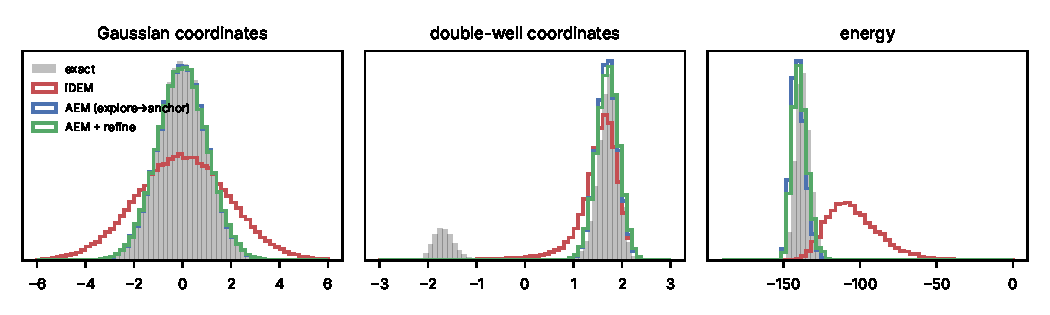
\includegraphics[width=\columnwidth]{fig_mw_marginals.pdf}
\caption{\textbf{MW-32 marginals} (samples pooled over 3 seeds) against exact samples (grey). iDEM's fixed-point bias widens the Gaussian coordinates and shifts the energy distribution. The anchored models remove both, but they concentrate the double-well coordinates in the major well.}
\label{fig:marginals}
\end{figure}

\paragraph{Other self-normalized targets.}
\Cref{tab:kinds} applies the consistency test to three self-normalized targets and their anchored versions, with the same draws as \cref{tab:diag} ($N=20\,000$; GMM-10 as a control with known score). TSI is the original iDEM target; DSI is the self-normalized posterior-mean estimate $\mathbb{E}[x_0\mid x_t]$, the form of the iEFM target in the VE parametrization; CV combines TSI and DSI with a per-point control-variate coefficient $\beta=\mathrm{Cov}_w(a,a-b)/\mathrm{Var}_w(a-b)$ estimated from the same weighted particles, in the spirit of CVSI~\citep{cvsi2025} (our implementation, not the authors'). All three unanchored targets are rejected at moderate and high noise. Anchoring fixes TSI and DSI, whose test functions are fixed. The anchored CV target is still rejected at some noise levels ($|z|$ up to $34$ on LJ-13): its coefficient depends on the particles, including the anchor, so \cref{thm:unbiased} does not apply. This is the bias we avoid by using the fixed schedule $\alpha_t$, and it shows that the test does have power against an anchored target when that target is biased.

\begin{table}[h]
\centering
\caption{Largest $|z|$ of the consistency test over the two test functions, for unanchored (iDEM-style) and anchored (AEM) versions of three self-normalized targets ($K=100$; bold: $|z|>3$; --: $T\equiv u$ exactly, so $z$ is undefined).}
\label{tab:kinds}
\small
\setlength{\tabcolsep}{3.5pt}
\begin{tabular}{lrcccccc}
\toprule
& & \multicolumn{3}{c}{unanchored} & \multicolumn{3}{c}{anchored}\\
\cmidrule(lr){3-5}\cmidrule(lr){6-8}
target & $\sigma_t$ & TSI & DSI & CV & TSI & DSI & CV\\
\midrule
DW-4 & 0.03 & 1.4 & 1.8 & 1.4 & 1.5 & 1.3 & 1.4\\
 & 0.1 & 0.7 & \textbf{3.6} & 1.0 & 1.5 & 1.2 & 1.4\\
 & 0.3 & \textbf{16.4} & \textbf{14.3} & \textbf{6.8} & 0.7 & 1.0 & 0.9\\
 & 1 & \textbf{25.1} & \textbf{18.1} & \textbf{21.7} & 0.9 & 2.2 & \textbf{7.6}\\
 & 2 & \textbf{30.1} & \textbf{35.4} & \textbf{3.3} & 0.2 & 0.3 & \textbf{5.1}\\
 & 3 & \textbf{39.4} & \textbf{49.1} & \textbf{15.1} & 0.4 & 0.8 & 0.5\\
\midrule
LJ-13 & 0.01 & 0.8 & 1.1 & 0.8 & 0.8 & 0.7 & 0.8\\
 & 0.03 & \textbf{3.2} & 1.6 & \textbf{3.2} & 1.2 & 0.7 & 1.3\\
 & 0.1 & \textbf{7.8} & \textbf{3.7} & \textbf{7.0} & 2.2 & 0.8 & 1.5\\
 & 0.3 & \textbf{7.6} & \textbf{31.2} & \textbf{19.5} & 1.3 & 1.2 & \textbf{3.8}\\
 & 1 & \textbf{39.0} & \textbf{213.8} & \textbf{141.8} & 1.5 & 1.6 & \textbf{30.2}\\
 & 2 & \textbf{111.3} & \textbf{355.6} & \textbf{97.9} & 0.9 & 1.5 & \textbf{34.1}\\
\midrule
GMM-10 & 3 & \textbf{258.8} & \textbf{245.6} & \textbf{4.5} & 0.9 & 1.0 & 0.8\\
 & 10 & \textbf{249.8} & \textbf{235.4} & \textbf{46.3} & 0.5 & -- & 0.5\\


\bottomrule
\end{tabular}
\end{table}

\paragraph{Combining TSI and DSI.}
Since every $g$ gives an unbiased target under the same particles and weights, any combination $\alpha_t g_{\mathrm{TSI}}+(1-\alpha_t)g_{\mathrm{DSI}}$ is also unbiased (\cref{thm:unbiased}).
We use the fixed schedule $\alpha_t=(1+\sigma_t^2)^{-1}$, which trusts TSI at low noise and DSI at high noise. For a target whose components are unit-covariance Gaussians, it makes the per-particle test function constant within a component, so the estimator has zero within-component variance. For other targets it is only a heuristic; a target-adapted choice would use the local curvature. Unlike the control-variate coefficient of \citet{cvsi2025}, it requires no per-batch estimation, which would reintroduce bias. Because this schedule favours unit-variance components, we give it to every method, iDEM included, and we check robustness to non-unit components in \cref{app:extra}.

\paragraph{Practical deviations from the theory.}
The exactness statements above concern the idealized estimator. Our implementation clips per-particle energy gradients and caps the norm of $\sigma_t\times$target, for stability and identically for all methods. Both are nonlinear and introduce a small bias. In addition, the buffer is a finite set of model samples that is reused across many steps, so even at convergence it is only approximately $\pi$.

